\subsection{Brakes}

The vehicle is turning by pulling the brakes, to slow down one side of the belts and then make the vehicle turn without changing the motor input velocity. An overview of one side of the brake can be seen in \figref{Brakes}. The servo, pulling the brakes, is explained later in \secref{Servo}.

 \begin{figure}[H]
	\centering
	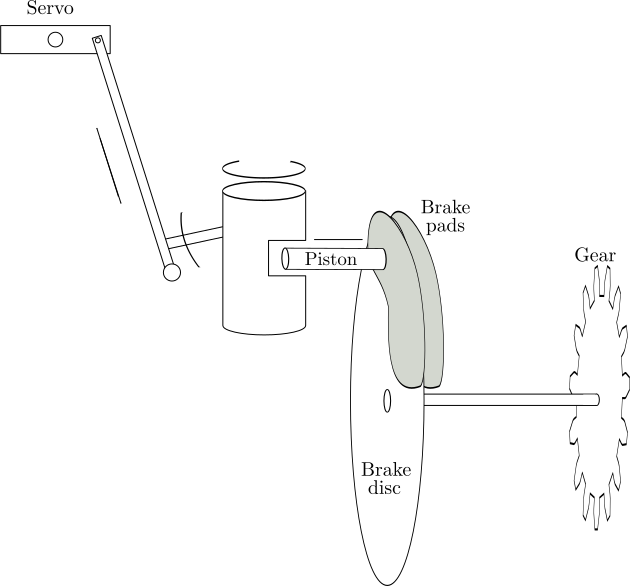
\includegraphics[scale=0.6]{figures/brakeDescription.pdf}
	\caption{Illustration of the brakes}
	\label{Brakes}
\end{figure}

When the servo turns on it self, it pulls an arm connected to a rotating cylinder, pushing a piston when it rotates. This piston push the brake pads one to each other. This will apply a friction on the brake disc, connected to the gear of the belts. The brakes can not be pulled simultaneously.\\

Now that the brakes are described, the servo pulling them will be described.